\documentclass[aspectratio=169, 12pt]{beamer}

% ─── Tema base ────────────────────────────────────────────────────────────────
\usetheme{Madrid}

% ─── Cores personalizadas ─────────────────────────────────────────────────────
\usepackage{xcolor}
\definecolor{azulP}{RGB}{0,82,155}
\definecolor{azulL}{RGB}{30,120,210}
\definecolor{cinza}{RGB}{60,60,60}
\definecolor{verde}{RGB}{39,174,96}
\definecolor{laranja}{RGB}{230,126,34}
\definecolor{fundo}{RGB}{245,248,252}
\definecolor{codebg}{RGB}{28,28,36}

\setbeamercolor{palette primary}{bg=azulP, fg=white}
\setbeamercolor{palette secondary}{bg=azulL, fg=white}
\setbeamercolor{palette tertiary}{bg=azulP, fg=white}
\setbeamercolor{palette quaternary}{bg=azulP, fg=white}
\setbeamercolor{structure}{fg=azulP}
\setbeamercolor{section in toc}{fg=azulP}
\setbeamercolor{block title}{bg=azulP, fg=white}
\setbeamercolor{block body}{bg=azulP!8, fg=cinza}
\setbeamercolor{alerted text}{fg=laranja}
\setbeamercolor{background canvas}{bg=fundo}
\setbeamercolor{example text}{fg=verde!70!black}
\setbeamercolor{block title example}{bg=verde!70!black, fg=white}
\setbeamercolor{block body example}{bg=verde!8, fg=cinza}

\setbeamerfont{title}{size=\Large,series=\bfseries}
\setbeamerfont{frametitle}{size=\large,series=\bfseries}
\setbeamerfont{block title}{series=\bfseries}

% ─── Pacotes ──────────────────────────────────────────────────────────────────
\usepackage[utf8]{inputenc}
\usepackage[T1]{fontenc}
\usepackage[portuguese]{babel}
\usepackage{listings}
\usepackage{tikz}
\usepackage{graphicx}
\usepackage{booktabs}
\usepackage{array}

\usetikzlibrary{arrows.meta,shapes.geometric,positioning,calc}

% ─── Estilos listings ─────────────────────────────────────────────────────────
\lstdefinestyle{cpp}{
  language=C++,
  basicstyle=\ttfamily\scriptsize\color{black},
  keywordstyle=\color{azulP}\bfseries,
  stringstyle=\color{laranja},
  commentstyle=\color{verde}\itshape,
  numberstyle=\tiny\color{gray},
  numbers=left, numbersep=5pt,
  breaklines=true, frame=none,
  tabsize=2, showstringspaces=false,
  morekeywords={String,byte,WiFiClient,PubSubClient,WiFiUDP,NTPClient,LeitorRFID}
}

\lstdefinestyle{python}{
  language=Python,
  basicstyle=\ttfamily\scriptsize\color{black},
  keywordstyle=\color{azulP}\bfseries,
  stringstyle=\color{laranja},
  commentstyle=\color{verde}\itshape,
  numberstyle=\tiny\color{gray},
  numbers=left, numbersep=5pt,
  breaklines=true, frame=none,
  tabsize=2, showstringspaces=false
}

\lstdefinestyle{bash}{
  basicstyle=\ttfamily\scriptsize\color{black},
  breaklines=true, frame=single, rulecolor=\color{cinza!30}, numbers=none,
  showstringspaces=false
}

\lstdefinestyle{json}{
  basicstyle=\ttfamily\scriptsize\color{black},
  stringstyle=\color{azulP},
  keywordstyle=\color{laranja},
  breaklines=true, frame=none, numbers=none,
  showstringspaces=false,
  morestring=[b]"
}

% ─── Navegação ────────────────────────────────────────────────────────────────
\setbeamertemplate{navigation symbols}{}
\setbeamertemplate{footline}[frame number]

% ─── Metadados ────────────────────────────────────────────────────────────────
\title[RFID via MQTT]{Sistema de Leitura RFID via MQTT}
\subtitle{Projeto de Automa\c{c}\~{a}o II}
\author{Tomás Espincho 110486}
\institute[UA]{Universidade de Aveiro}
\date{\today}

% ══════════════════════════════════════════════════════════════════════════════
\begin{document}

%──────────────────────────────────────────────────────────────────────────────
% SLIDE 1: TÍTULO
%──────────────────────────────────────────────────────────────────────────────
\begin{frame}
  \titlepage
  \begin{tikzpicture}[remember picture,overlay]
    \fill[azulP!12] (current page.south west) rectangle ++(16,0.7);
    \node[anchor=south west, font=\scriptsize, text=azulP!70]
    at ($(current page.south west)+(0.3,0.1)$)
    {ESP32 \textbullet\ RFID \textbullet\ MQTT \textbullet\ Python \textbullet\ Docker};
  \end{tikzpicture}
\end{frame}

%──────────────────────────────────────────────────────────────────────────────
% SLIDE 2: ÍNDICE
%──────────────────────────────────────────────────────────────────────────────
\begin{frame}{\'{I}ndice}
  \tableofcontents[hideallsubsections]
\end{frame}

%──────────────────────────────────────────────────────────────────────────────
\section{Introdu\c{c}\~{a}o e Objetivos}
%──────────────────────────────────────────────────────────────────────────────
\begin{frame}{Introdu\c{c}\~{a}o e Objetivos}
  \begin{columns}[T]
    \begin{column}{0.56\textwidth}
      \begin{block}{Objetivo Principal}
        Desenvolver um projeto capaz de \textbf{ler tags RFID}
        e \textbf{transmitir dados em tempo real} via MQTT.
      \end{block}
      \vspace{0.4em}
      \begin{block}{Objetivos Espec\'{i}ficos}
        \begin{itemize}
          \item Capturar o UID de cart\~{o}es RFID com ESP32
          \item Sincronizar tempo via NTP
          \item Publicar dados JSON no broker MQTT
          \item Receber e processar os dados
          \item Simular leituras sem hardware f\'{i}sico
        \end{itemize}
      \end{block}
    \end{column}
    \begin{column}{0.41\textwidth}
      \vspace{1cm}
      \hspace{0.5cm}
      \begin{tikzpicture}
        \node[draw=azulP, fill=azulP!8, rounded corners=6pt,
        minimum width=5cm, minimum height=3.5cm, thick] (caixa) {};
        \node[font=\small\bfseries, text=azulP, above=-0.1cm of caixa.north]
        at ($(caixa.north)+(0,-0.5)$) {Casos de Uso};
        \foreach \i/\txt/\cor in {
          0/{Controlo de Acessos}/verde,
          1/{Controlo de inventário}/laranja%
        }{
          \node[draw=\cor, fill=\cor!12, rounded corners=4pt,
          minimum width=4.4cm, minimum height=0.75cm,
          font=\small\bfseries, text=\cor!75!black]
          at ($(caixa.north)+(0,-1.2-\i*1.5)$) {\txt};
        }
      \end{tikzpicture}
    \end{column}
  \end{columns}
\end{frame}

%──────────────────────────────────────────────────────────────────────────────
\section{Arquitetura do Sistema}
%──────────────────────────────────────────────────────────────────────────────
\begin{frame}[fragile]{Arquitetura do Sistema}
  \centering
  \begin{tikzpicture}[
    node distance=1.6cm and 2.0cm,
    caixa/.style={draw=#1,fill=#1!12,rounded corners=5pt,
      minimum width=2.3cm,minimum height=1.0cm,
    font=\small\bfseries,text=#1!75!black,thick,align=center},
    seta/.style={-{Latex[length=3mm]},thick,color=#1}
    ]
    \node[caixa=verde]   (tag)    {Tag\\RFID};
    \node[caixa=azulL,   right=1.2cm of tag]    (esp)    {ESP32\\+LeitorRFID};
    \node[caixa=azulP,   right=2.1cm of esp]    (broker) {Broker\\MQTT};
    \node[caixa=laranja, right=of broker] (py)     {Python\\Receiver};

    \draw[seta=verde]  (tag)    -- node[above,font=\tiny\itshape,gray]{} (esp);
    \draw[seta=azulL]  (esp)    -- node[above,font=\tiny\itshape,gray]{WiFi/TCP Publish}   (broker);
    \draw[seta=azulP]  (broker) -- node[above,font=\tiny\itshape,gray]{Subscribe}  (py);

    % NTP
    \node[draw=cinza!50, fill=cinza!8, rounded corners=3pt,
    minimum width=2.0cm, minimum height=0.7cm,
    font=\tiny\bfseries, text=cinza, above=1.0cm of esp] (ntp) {NTP Server};
    \draw[-{Latex},cinza!60,dashed,thick] (ntp) -- node[right,font=\tiny\itshape]{tempo} (esp);

    % Log
    \node[draw=verde!60, fill=verde!8, rounded corners=3pt,
    minimum width=2.0cm, minimum height=0.7cm,
    font=\tiny\bfseries, text=verde!70!black, above=1.0cm of py] (log) {logs\_rfid.jsonl};
    \draw[-{Latex},verde!60,dashed,thick] (py) -- (log);

    % Docker badge
    \node[draw=azulL!50, fill=azulL!8, rounded corners=3pt,
    font=\tiny, text=azulL!80!black,
    below=0.4cm of broker, minimum width=2.3cm] {Docker Container};

    % Topico badge
    \node[draw=laranja!50, fill=laranja!8, rounded corners=3pt,
    font=\tiny, text=laranja!80!black,
    below=0.4cm of py, minimum width=2.7cm] {aii/projeto/rfid};
  \end{tikzpicture}

  \vspace{0.5em}
  \begin{columns}
    \column{.33\textwidth}\centering
    {\footnotesize\color{verde}\textbf{Hardware}\\Tag + Leitor RFID}
    \column{.33\textwidth}\centering
    {\footnotesize\color{azulL}\textbf{Transporte}\\WiFi + MQTT}
    \column{.33\textwidth}\centering
    {\footnotesize\color{laranja}\textbf{Aplica\c{c}\~{a}o}\\Python + JSON}
  \end{columns}
\end{frame}

%──────────────────────────────────────────────────────────────────────────────
\section{Hardware}
%──────────────────────────────────────────────────────────────────────────────
\begin{frame}{Hardware -- ESP32 e M\'{o}dulo RFID}
  \begin{columns}[T]
    \begin{column}{0.48\textwidth}
      \centering
      % Imagem do esquemático
      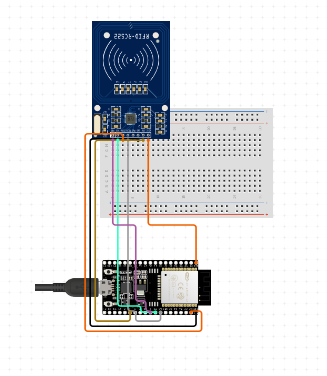
\includegraphics[width=\textwidth,height=5cm,keepaspectratio]{img/esquema.png}
    \end{column}

    \begin{column}{0.48\textwidth}
      \begin{block}{Fun\c{c}\~{a}o das Entradas RFID}
        \begin{itemize}\setlength{\itemsep}{2pt}
          \footnotesize
          \item \textbf{3.3V / GND:} Alimentação.
          \item \textbf{RST (Pino 4):} Reset f\'{i}sico e \textit{power-down}.
          \item \textbf{NSS (Pino 5):} Seleção do Slave SPI.
          \item \textbf{SCK (Pino 18):} Sinal de Clock do SPI.
          \item \textbf{MISO (Pino 19):} Sa\'{i}da de dados do leitor para o ESP32.
          \item \textbf{MOSI (Pino 23):} Entrada de dados do ESP32 para o leitor.
        \end{itemize}
      \end{block}
    \end{column}  \end{columns}
  \end{frame}

  %──────────────────────────────────────────────────────────────────────────────
  \section{Programa ESP32}
  %──────────────────────────────────────────────────────────────────────────────
  \begin{frame}[fragile]{Programa ESP32 -- Leitura e Publica\c{c}\~{a}o}
    \begin{columns}[T]
      \begin{column}{0.55\textwidth}
        \begin{block}{Excerto do Loop Principal}
          \begin{lstlisting}[style=cpp]
// 1. Ler e formatar UID (ex: "A1B2C3D4")
String tagUID = readAndFormatUID();

// 2. Obter Timestamp (NTP)
unsigned long ts = timeClient.getEpochTime();

// 3. Construir Payload JSON
String payload = "{\"dispositivo\" : \"Esp32\",
    \"uid\": \"" + finalUID + "\",
    \"timestamp\": \"" + String(timeStamp) + "\"}";
// 4. Publicar no Broker
client.publish("aii/projeto/rfid", payload.c_str());
          \end{lstlisting}
        \end{block}
      \end{column}
      \begin{column}{0.43\textwidth}
        \begin{block}{Fluxo do programa}
          \begin{tikzpicture}[
            passo/.style={draw=azulP,fill=azulP!10,rounded corners=3pt,
              minimum width=3.6cm,minimum height=0.55cm,
            font=\scriptsize,text=azulP!80!black,align=center},
            seta/.style={-{Latex},azulP,thick}
            ]
            \node[passo]                            (w) {1. Ligar ao WiFi};
            \node[passo,below=0.28cm of w]          (n) {2. Sincronizar NTP};
            \node[passo,below=0.28cm of n]          (m) {3. Ligar ao Broker};
            \node[passo,below=0.28cm of m,
            draw=verde,fill=verde!10,
            text=verde!70!black]              (r) {4. Aguardar Tag RFID};
            \node[passo,below=0.28cm of r,
            draw=laranja,fill=laranja!10,
            text=laranja!80!black]            (p) {5. Publicar JSON};
            \node[passo,below=0.28cm of p]          (h) {6. Espera para não ler 2 vezes};

            \draw[seta] (w)--(n);
            \draw[seta] (n)--(m);
            \draw[seta] (m)--(r);
            \draw[seta] (r)--(p);
            \draw[seta] (p)--(h);
            \draw[seta] (h.east)
            .. controls +(0.9,0) and +(0.9,0) ..
            node[midway, right, font=\tiny\bfseries, text=cinza] {Loop Principal}
            (r.east);
          \end{tikzpicture}
        \end{block}
      \end{column}
    \end{columns}
  \end{frame}

  %──────────────────────────────────────────────────────────────────────────────
  \section{Protocolo MQTT e Broker}
  %──────────────────────────────────────────────────────────────────────────────
  \begin{frame}[fragile]{Protocolo MQTT e Infraestrutura}
    \begin{columns}[T]
      \begin{column}{0.48\textwidth}
        \begin{block}{O que \'{e} o MQTT?}
          \textbf{Message Queuing Telemetry Transport}
          \begin{itemize}
            \item Protocolo \textbf{pub/sub}
            \item Leve em termos de dados
            \item Baseado em \textbf{t\'{o}picos}
          \end{itemize}
        \end{block}
        \vspace{0.4em}
        \begin{block}{T\'{o}pico Utilizado}
          \centering
          \large\texttt{\textbf{aii/projeto/rfid}}\\[0.3em]
          \footnotesize Publisher: ESP32 \quad|\quad Subscriber: Python
        \end{block}
      \end{column}
      \begin{column}{0.50\textwidth}
        \begin{block}{Broker -- Eclipse Mosquitto}
          \begin{itemize}
            \item Utilizado para testes locais 
            \item Executado localmente via \textbf{Docker}
          \end{itemize}
        \end{block}
        \vspace{0.3em}
        \begin{exampleblock}{docker-compose.yml}
          \begin{lstlisting}[style=bash]
services:
mosquitto:
image: eclipse-mosquitto:latest
ports:
- "1883:1883"
volumes:
- ./conf/mosquitto.conf:
/mosquitto/config/
mosquitto.conf
          \end{lstlisting}
        \end{exampleblock}
      \end{column}
    \end{columns}
  \end{frame}

  %──────────────────────────────────────────────────────────────────────────────
  \section{Scripts Python}
  %──────────────────────────────────────────────────────────────────────────────
  \begin{frame}[fragile]{Scripts Python -- Recetor e Simulador}
    \begin{columns}[T]
      \begin{column}{0.49\textwidth}
        {\color{azulP}\textbf{reciver.py}} -- Recetor MQTT
        \begin{lstlisting}[style=python]
def on_message(client, userdata, msg):
dados = json.loads(msg.payload.decode())
print(f"TAG LIDA: {dados.get('uid')}")

# Setup e Subscricao
client = mqtt.Client()
client.on_message = on_message
client.connect(BROKER, PORT)
client.subscribe("aii/projeto/rfid")
client.loop_forever()
        \end{lstlisting}
      \end{column}
      \begin{column}{0.49\textwidth}
        {\color{laranja}\textbf{sender.py}} -- Simulador
        \begin{lstlisting}[style=python]
while True:
payload = json.dumps({
  "dispositivo": "Esp32",
  "uid": "A1B2C3D4",
  "timestamp": int(time.time())
})

client.publish("aii/projeto/rfid", payload)
time.sleep(random.randint(3,8))      
        \end{lstlisting}
        \vspace{0.2em}
        \begin{exampleblock}{Configura\c{c}\~{a}o .env}
          \begin{lstlisting}[style=bash]
MQTT_BROKER=192.168.1.100
MQTT_PORT=1883
          \end{lstlisting}
        \end{exampleblock}
      \end{column}
    \end{columns}
  \end{frame}

  %──────────────────────────────────────────────────────────────────────────────
  \section{Formato de Dados}
  %──────────────────────────────────────────────────────────────────────────────
  \begin{frame}[fragile]{Formato de Dados -- JSON}
    \begin{columns}[T]
      \begin{column}{0.48\textwidth}
        \begin{block}{Payload do ESP32 (hardware)}
          \begin{lstlisting}[style=json]
{
  "dispositivo": "Esp32",
  "uid": "A1 B2 C3 D4",
  "timestamp": "1748900000"
}
          \end{lstlisting}
        \end{block}
        \vspace{0.4em}
        \begin{block}{Payload do Simulador Python}
          \begin{lstlisting}[style=json]
{
  "dispositivo": "Esp32",
  "uid": "A1B2C3D4",
  "timestamp": 1748900000
}
          \end{lstlisting}
        \end{block}
      \end{column}
      \begin{column}{0.50\textwidth}
        \vspace{0.4em}
        \begin{alertblock}{Persist\^{e}ncia}
          O ficheiro \texttt{logs\_rfid.jsonl} pode ser ativado no recetor para guardar todas as leituras no disco.
        \end{alertblock}
      \end{column}
    \end{columns}
  \end{frame}

  %──────────────────────────────────────────────────────────────────────────────
  \section{Conclus\~{a}o}
  %──────────────────────────────────────────────────────────────────────────────
  \begin{frame}{Conclus\~{a}o e Pr\'{o}ximos Passos}
    \begin{columns}[T]
      \begin{column}{0.50\textwidth}
        \begin{block}{O que foi implementado}
          \begin{itemize}
            \item[$\checkmark$] Leitura de tags RFID (ESP32 + LeitorRFID)
            \item[$\checkmark$] Sincroniza\c{c}\~{a}o de tempo via NTP
            \item[$\checkmark$] Publica\c{c}\~{a}o de JSON via MQTT
            \item[$\checkmark$] Broker local com Docker (Mosquitto)
            \item[$\checkmark$] Recetor Python
            \item[$\checkmark$] Simulador para testes sem hardware
            \item[$\checkmark$] Dashboard (Node-RED / html)
          \end{itemize}
        \end{block}
      \end{column}
      \begin{column}{0.48\textwidth}
        \begin{alertblock}{Poss\'{i}veis Extens\~{o}es}
          \begin{itemize}
            \item Base de dados (InfluxDB / SQLite)
            \item Controlo de acesso com lista de UIDs
            \item Autentica\c{c}\~{a}o MQTT com TLS
            \item M\'{u}ltiplos leitores em paralelo
          \end{itemize}
        \end{alertblock}
      \end{column}
    \end{columns}
    \vspace{0.7em}
    \centering
    \begin{tikzpicture}
      \node[draw=azulP,fill=azulP!10,rounded corners=6pt,
      minimum width=11cm,minimum height=0.9cm,
      font=\normalsize\bfseries,text=azulP]
      {Tag RFID $\rightarrow$ ESP32 $\rightarrow$ MQTT $\rightarrow$ Python / NodeRed};
    \end{tikzpicture}
  \end{frame}

  %──────────────────────────────────────────────────────────────────────────────
  \section{Demonstra\c{c}\~{a}o}
  %──────────────────────────────────────────────────────────────────────────────
  \begin{frame}{Demonstra\c{c}\~{a}o ao Vivo}
    \begin{columns}[T]
      \begin{column}{0.95\textwidth}
        \begin{block}{O que vamos mostrar}
          \begin{enumerate}
            \item \textbf{Recetor Python} --- Escuta de mensagens no t\'{o}pico \texttt{aii/projeto/rfid}
            \item \textbf{ESP32 + Leitor RFID} --- Leitura de tags f\'{i}sicas e publica\c{c}\~{a}o de dados
            \item \textbf{Simulador Python} --- Inje\c{c}\~{a}o de leituras virtuais
          \end{enumerate}
        \end{block}
        \vspace{0.4em}
      \end{column}
    \end{columns}
  \end{frame}

  %──────────────────────────────────────────────────────────────────────────────
  % SLIDE FINAL
  %──────────────────────────────────────────────────────────────────────────────
  \begin{frame}{Slide Final}
    \begin{tikzpicture}[remember picture,overlay]
      \fill[azulP] (current page.south west) rectangle (current page.north east);
    \end{tikzpicture}
    \centering
    \vspace{1.8em}
    {\Huge\bfseries\color{white} Obrigado!}\\[1.0em]
    {\large\color{white!80} Projeto de Automa\c{c}\~{a}o II}\\[2.0em]
    \vspace{1.2em} 
    {\color{white!60}\small Quest\~{o}es?}
  \end{frame}

  \end{document}
